\documentclass[tikz,border=10pt]{standalone}
\usepackage{tikz}
\usetikzlibrary{shapes,arrows,positioning,fit}

\begin{document}
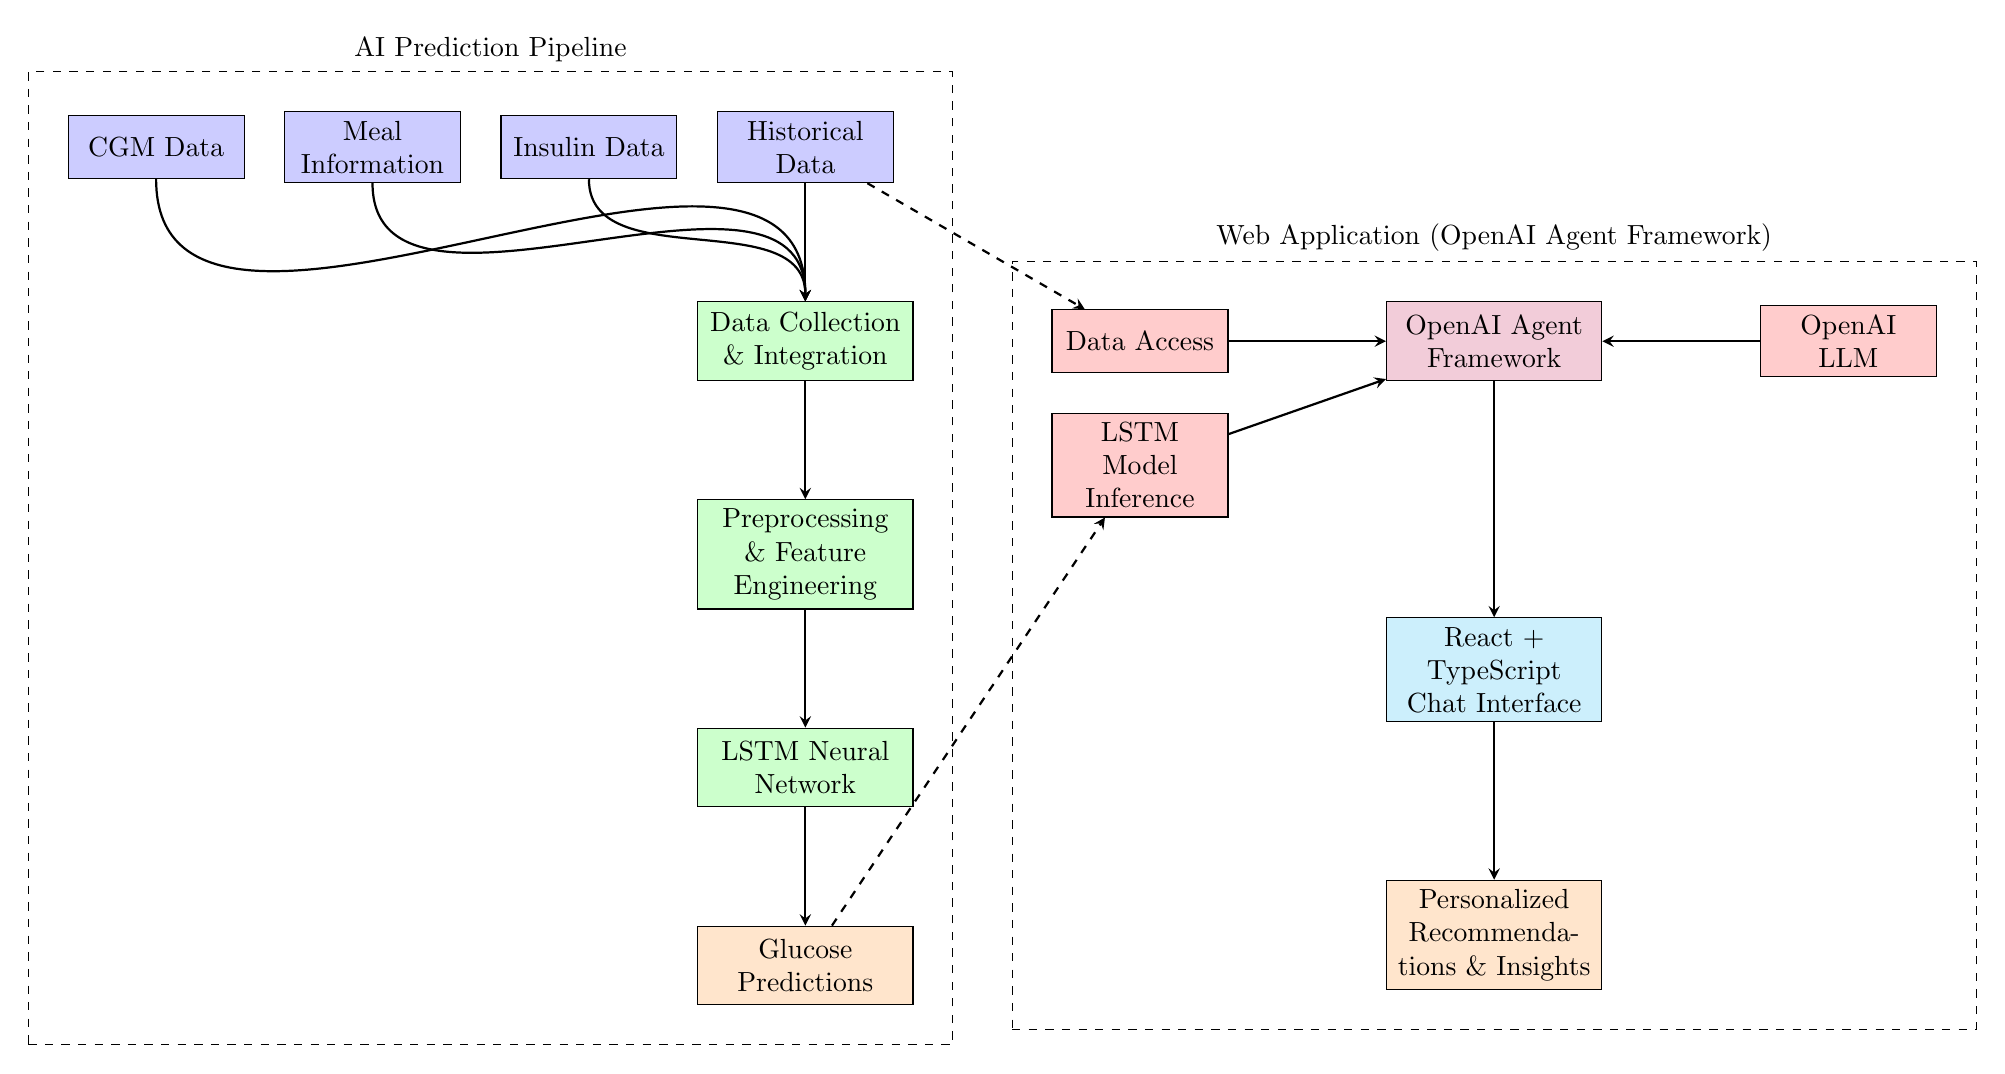
\begin{tikzpicture}[
    node distance=2cm,
    box/.style={rectangle, draw, text width=2.5cm, text centered, minimum height=1cm, rounded corners},
    arrow/.style={thick,->,>=stealth},
    data/.style={rectangle, draw, fill=blue!20, text width=2cm, text centered, minimum height=0.8cm},
    process/.style={rectangle, draw, fill=green!20, text width=2.5cm, text centered, minimum height=1cm},
    output/.style={rectangle, draw, fill=orange!20, text width=2.5cm, text centered, minimum height=1cm},
    agent/.style={rectangle, draw, fill=purple!20, text width=2.5cm, text centered, minimum height=1cm},
    tool/.style={rectangle, draw, fill=red!20, text width=2cm, text centered, minimum height=0.8cm},
    ui/.style={rectangle, draw, fill=cyan!20, text width=2.5cm, text centered, minimum height=1cm},
    group/.style={rectangle, draw, dashed, inner sep=0.5cm}
  ]


  % AI Prediction Pipeline (Left side - Vertical)
  \node[data] (cgm) {CGM Data};
  \node[data, right=0.5cm of cgm] (meals) {Meal Information};
  \node[data, right=0.5cm of meals] (insulin) {Insulin Data};
  \node[data, right=0.5cm of insulin] (history) {Historical Data};

  % Data collection
  \node[process, below=1.5cm of history] (collect) {Data Collection \& Integration};

  % Preprocessing
  \node[process, below=1.5cm of collect] (preprocess) {Preprocessing \& Feature Engineering};

  % LSTM Model
  \node[process, below=1.5cm of preprocess] (lstm) {LSTM Neural Network};

  % Model Output
  \node[output, below=1.5cm of lstm] (predictions) {Glucose Predictions};

  % Group the AI pipeline
  \node[group, fit=(cgm)(meals)(history)(collect)(preprocess)(lstm)(predictions), label=above:AI Prediction Pipeline] (ai_pipeline) {};

  % Web App with OpenAI Agent Framework (Right side)
  \node[agent, right=6cm of collect] (openai_agent) {OpenAI Agent Framework};

  % Available tools for the agent
  \node[tool, left=2cm of openai_agent] (data_tool) {Data Access};
  \node[tool, below=0.5cm of data_tool] (model_tool) {LSTM Model Inference};
  \node[tool, right=2cm of openai_agent] (open_ai_llm_tool) {OpenAI LLM};


  % Chat UI Technology Stack
  \node[ui, below=3cm of openai_agent] (chat_ui) {React + TypeScript Chat Interface};


  % Final output
  \node[output, below=2cm of chat_ui] (recommendations) {Personalized Recommendations \& Insights};

  % Arrows for AI pipeline (vertical flow)
  \draw[arrow] (cgm) to[out=270, in=90] (collect);
  \draw[arrow] (meals) to[out=270, in=90] (collect);
  \draw[arrow] (history) to[out=270, in=90] (collect);
  \draw[arrow] (insulin) to[out=270, in=90] (collect);
  \draw[arrow] (collect) -- (preprocess);
  \draw[arrow] (preprocess) -- (lstm);
  \draw[arrow] (lstm) -- (predictions);

  % Arrows connecting AI pipeline to web app
  \draw[arrow, dashed] (predictions) -- (model_tool);
  \draw[arrow, dashed] (history) -- (data_tool);

  % Arrows for agent framework
  \draw[arrow] (model_tool) -- (openai_agent);
  \draw[arrow] (data_tool) -- (openai_agent);
  \draw[arrow] (open_ai_llm_tool) -- (openai_agent);


  % Arrows for chat UI
  \draw[arrow] (openai_agent) -- (chat_ui);
  \draw[arrow] (chat_ui) -- (recommendations);

  % Group the web app
  \node[group, fit=(openai_agent)(model_tool)(data_tool)(open_ai_llm_tool)(chat_ui)(recommendations), label=above:Web Application (OpenAI Agent Framework)] (web_app) {};

\end{tikzpicture}
\end{document}
